\documentclass[letterpaper,11pt]{article}
\usepackage[top=1in, bottom=1.25in, left=1.25in, right=1.25in]{geometry}
\usepackage{graphicx} % in order to include graphics
% \usepackage{epstopdf} % when one wants to input .eps files
\usepackage{epstopdf} % conversion of eps to pdf files for pdflatex
\usepackage{textcomp} % for some macros such as textcelsius or textdegree
\usepackage[retainorgcmds]{IEEEtrantools} % for use of IEEEeqnarray
% \begin{IEEEeqnarray*}{rCl}
% \IEEEyesnumber
% \IEEEnonumber
% \end{IEEEeqnarray*}
\usepackage{amsmath} % for nice mathematical typsetting
\usepackage{amssymb} % for other symbols, including \triangleq
\usepackage{url}     % formats urls in the text
\usepackage{siunitx} % allows formatting of numbers and units
% tikz package and libraries in localtexmf
%  \usepackage{tikz}    % drawing package for shapes
%  \usetikzlibrary{shapes,arrows} % tikz library
%  \usetikzlibrary{dsp,chains}
%  \usepackage{signalflowdiagram}
% template for including pdf graphics
% trim order is left, bottom, right, top
% default units are bp (big points = 1/72 inch)
%\begin{center}
%	\begin{figure}[tbph]
%		\centering
%		\includegraphics[trim= 3.75cm 8.8cm 3.35cm 8.5cm,clip,width=0.95\linewidth]{graphicsDir/grahpicsFile.pdf}
%		\caption[myCaptionLabel]{This is my caption.}
%		\label{fig:myFigureLabel}
%	\end{figure}
%\end{center}
\DeclareSIUnit{\dBm}{dBm}
\DeclareSIUnit{\dBc}{dBc}

\author{J.~Sebek}
\title{Preliminary Comparison of LLRF9 with the Legacy LLRF System}
\begin{document}
	\maketitle
%	\tableofcontents

\section{Introduction}
In early 2021 we, Dmitry Teytelman, Filippos Toufexis, John Wachter, and I, tested the Dimtel LLRF9 low level radio frequency (LLRF) controller on SPEAR3 in order to compare its performance with the existing LLRF system and evaluate its suitability to control SPEAR3.  This note presents results of measurements of the power spectrum measured in Cavity A, one of the four SPEAR3 cavities.

\section{Setup}
Prior to our tests we inserted \SI{20}{\dB} couplers upstream of the legacy LLRF system for all of the signals that we wanted the LLRF9 to monitor.  The addition of these couplers added an insertion loss of approximately \SI{0.4}{\dB} for the legacy system.  This insertion loss was accounted for by modifying existing constants in the legacy system.  We connected nine coupled signals to LLRF9, the klystron forward power, the forward powers to the four cavities and the cell probes of the four cavities.  Appropriate attenuators were added to these coupled signals in order to bring their signal power down to the desired input power levels for the LLRF9.

In order to provide additional external monitoring points, we added \SI{3}{\dB} power splitters to several of the coupled signals before they entered the LLRF9.  The only second port of these splitters that was measured in operation was that of the Cavity A probe.  All unused ports were terminated.  The Cavity A probe signal was connected to a Rohde \& Schwarz FSW13 spectrum analyzer.  We set the span of the analyzer to \SI{50}{\kHz} and its resolution and video bandwidths to \SI{1}{\Hz}.  The blue trace in figure \ref{fig:legacyTotal} shows a typical spectrum using the legacy system to control the RF system with \SI{500}{\mA} in the ring.

\begin{center}
	\begin{figure}[tbph]
		\centering
		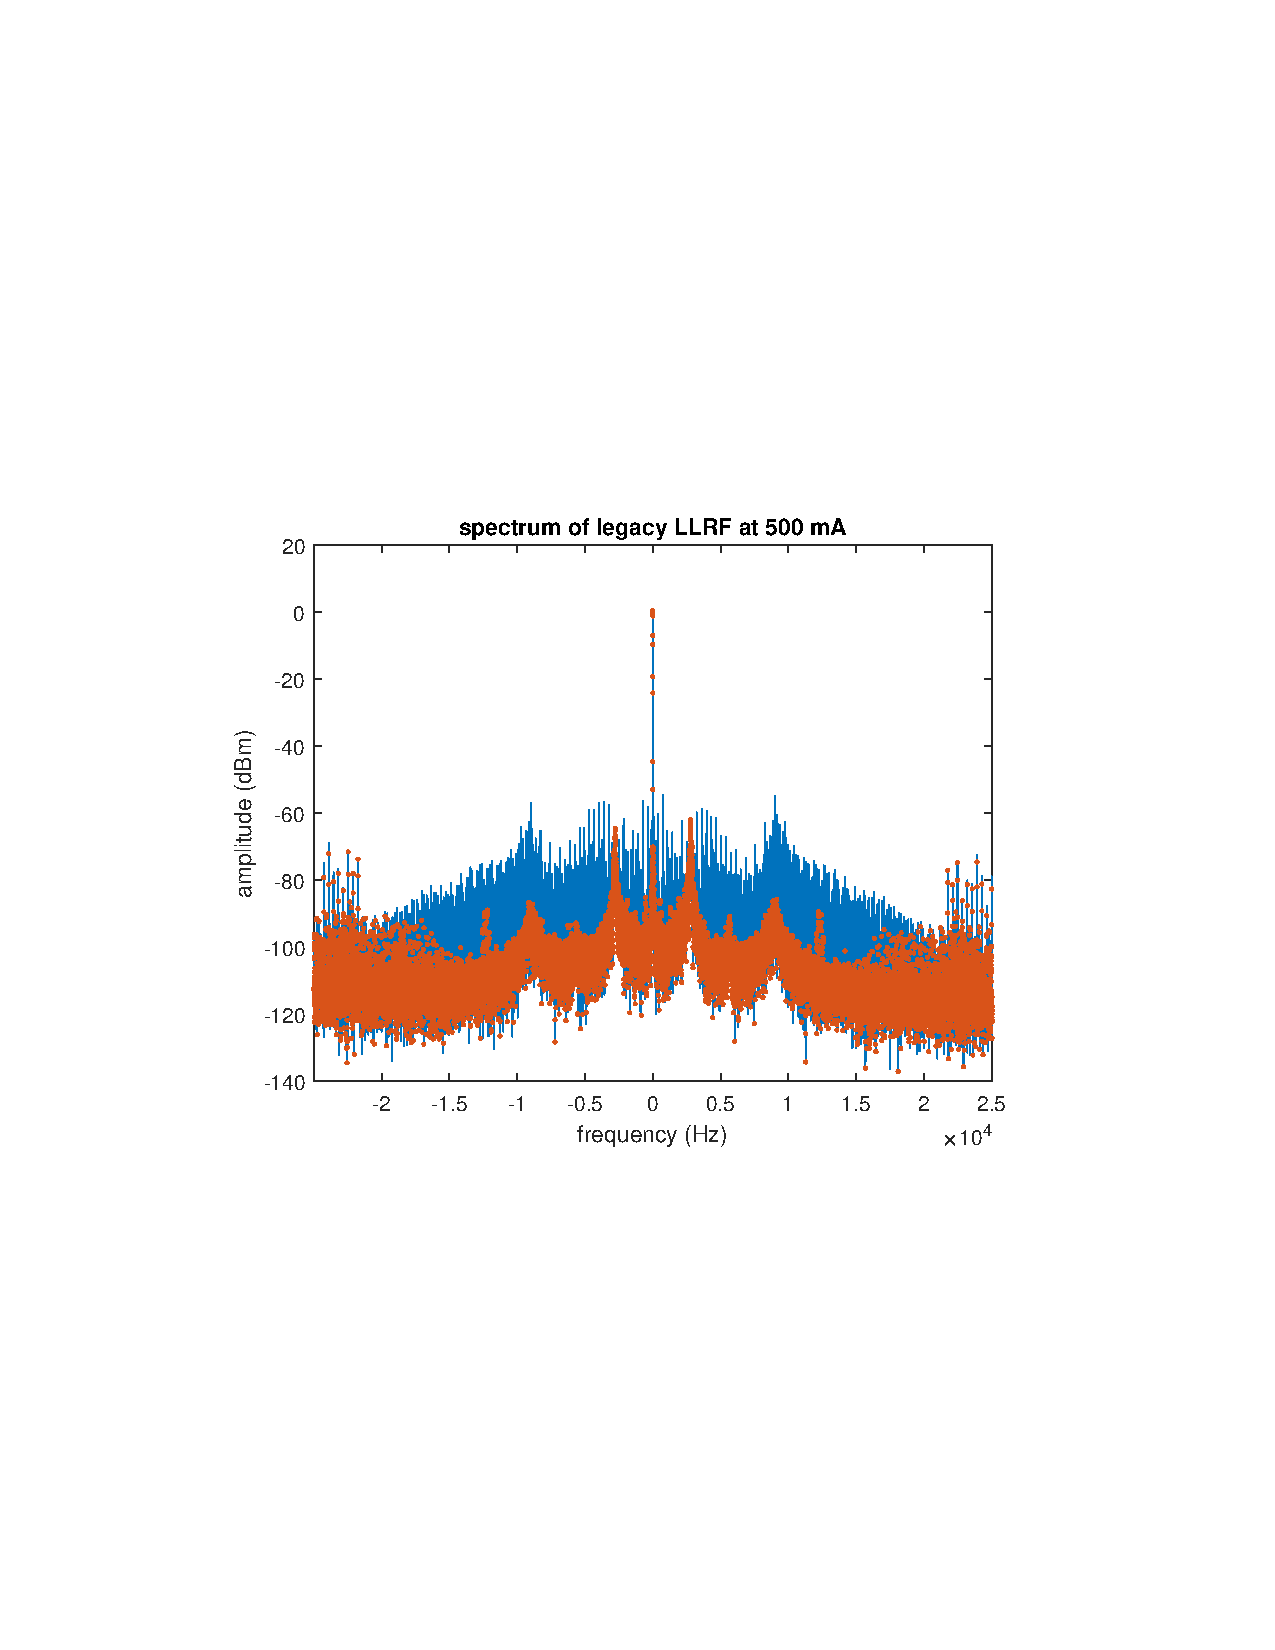
\includegraphics[trim= 3.75cm 8.5cm 3.35cm 8.5cm,clip,width=0.95\linewidth]{graphics/spearLegacy500Total.pdf}
		\caption[legacyTotal]{Unfiltered and filtered Cavity A spectrum with \SI{500}{\mA} using the legacy LLRF system.}
		\label{fig:legacyTotal}
	\end{figure}
\end{center}

\section{Filtering the Spectrum Analyzer Signal}
Because of klystron protection issues the klystron high voltage power supply (HVPS) contains many power line related harmonics.  These harmonics modulate the klystron output, both in amplitude and phase, and create sidebands of the fundamental RF carrier.  A detailed examination of the analyzer spectrum showed that although the principle sidebands were multiples of \SI{360}{\Hz} and \SI{720}{\Hz}, any multiple of \SI{30}{\Hz} could potentially be a narrow sideband measured by the analyzer.

It is important for the SPEAR3 LLRF system to suppress these sidebands as much as possible, but the main function of any SPEAR3 LLRF system is to control the RF field in the cavity while maximizing the beam stability.  That is, the LLRF should be tuned such that it damps out any potential synchrotron oscillations of the beam to acceptably low levels.  Physics studies of the beam showed that the power line harmonics can be seen on the beam, but they do not contribute to the instability of the synchrotron motion.  Therefore in order to accurately measure the spectrum of the residual synchrotron oscillations, we need to process the analyzer data through a software filter to remove these sidebands.

We implemented a simple and straightforward filter that partitioned the spectrum in segments of \SI{15}{\Hz}.  We removed \SI{15}{\Hz} of data centered on each sideband that was a multiple of \SI{30}{\Hz} and kept all of the rest of the data, including the fundamental frequency.  Figure \ref{fig:fswMask} shows an expanded view of a section of figure \ref{fig:legacyTotal}.  Data points are measured for every \SI{1}{\Hz}.  The blue trace connects these data points while, in order to avoid clutter, the orange trace does not.  We see that the filtered data avoids the power line harmonics.  With this filter we still get very good spectral coverage of the frequencies of interest while avoiding all of the power line generated sidebands.
\begin{center}
	\begin{figure}[tbph]
		\centering
		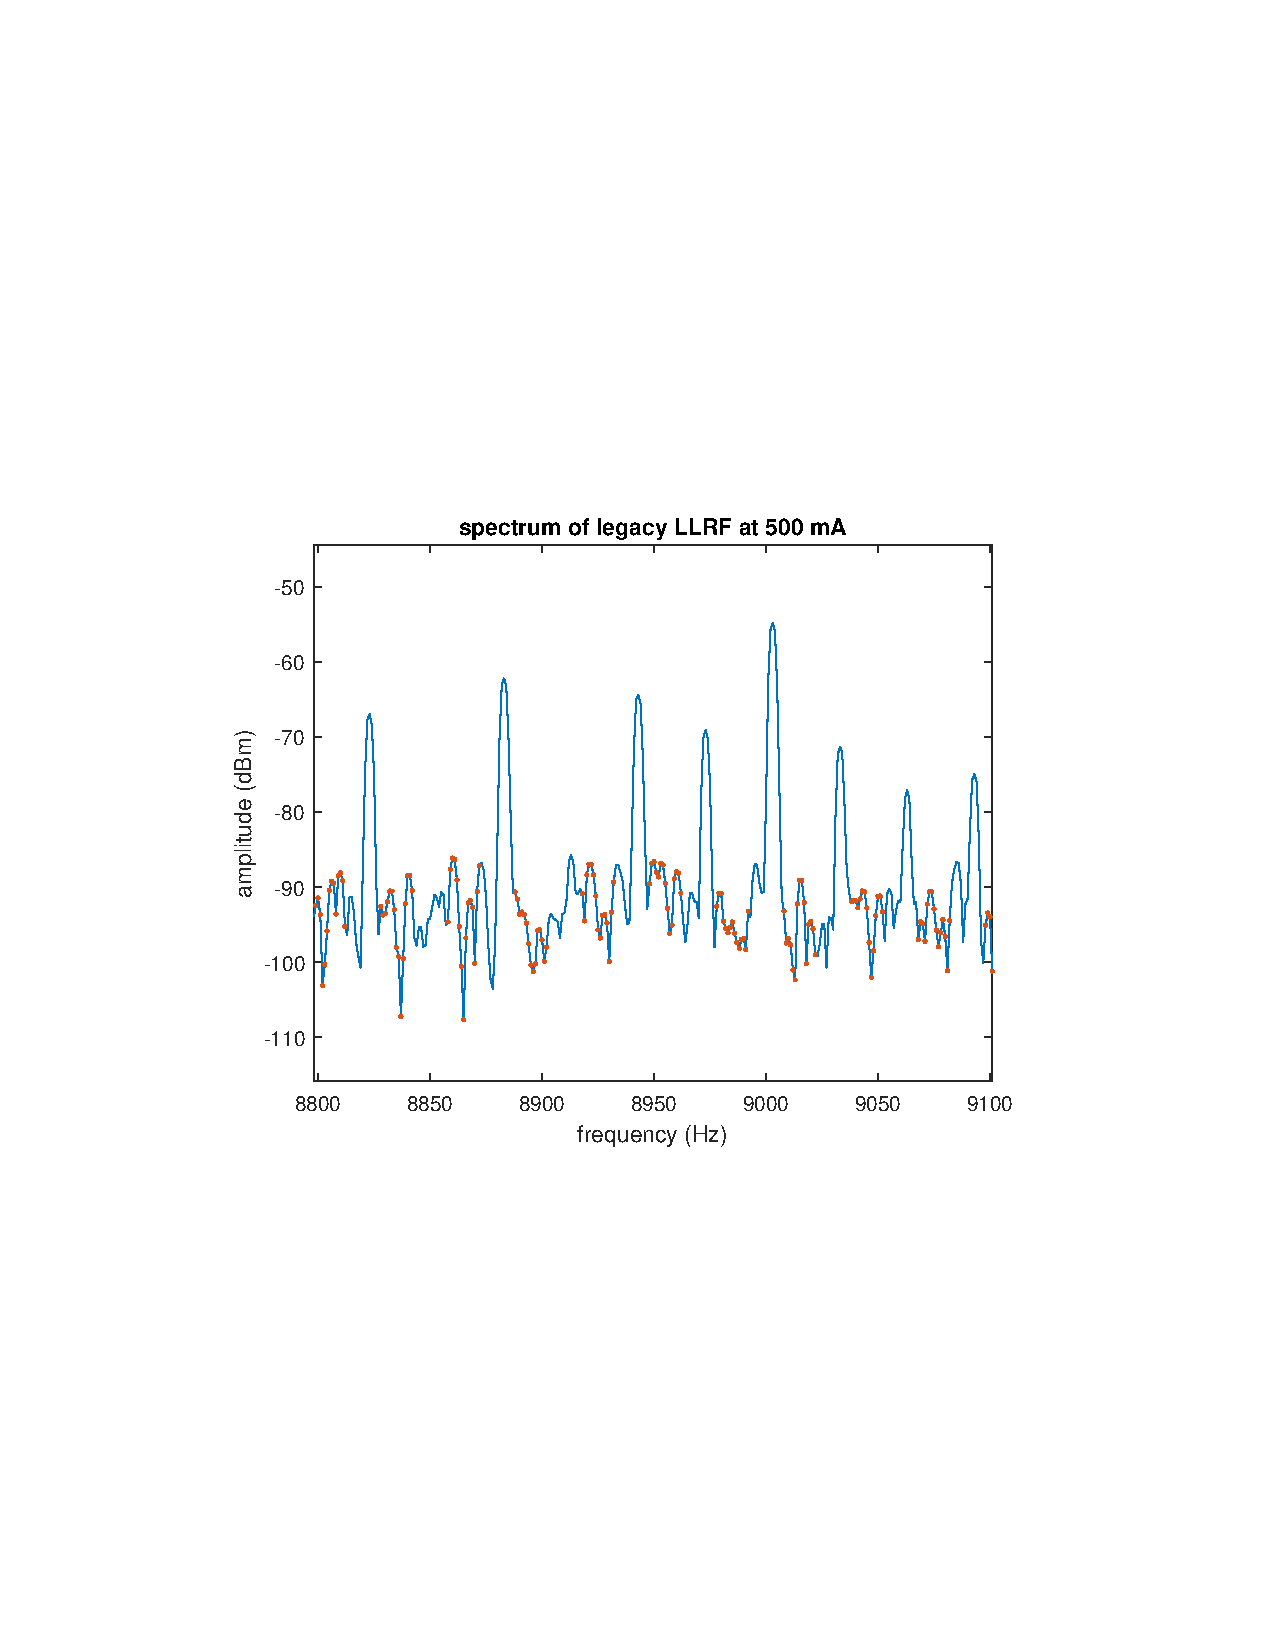
\includegraphics[trim= 3.75cm 8.5cm 3.35cm 8.5cm,clip,width=0.95\linewidth]{graphics/spearFswMask.pdf}
		\caption[fswMask]{Data around \(\nu_{s}\) showing the filter that notches out the \SI{30}{\hertz} harmonics.}
		\label{fig:fswMask}
	\end{figure}
\end{center}
\subsection{Raw Klystron Output Power}
As a measure of the effectiveness of this signal processing we look at the data from the raw RF output of the klystron, when no feedback from either LLRF system was used.  For these measurements, the gap voltage of the RF system was at its nominal value of \SI{2850}{\kV}, but the power was at about half of its nominal value since these measurements were taken with no beam in SPEAR.  From this data we can obtain the amplitude of the power line modulated sidebands introduced by the HVPS.  Figure \ref{fig:rawData} shows the raw data and the forest of sidebands which are down only about \SI{30}{\dBc} from the carrier.  Figure \ref{fig:rawDataFiltered} shows the effectiveness of our software filter in removing the harmonics from this data.  It also shows that there is no structure on the RF output other than the power line modulated sidebands.
\begin{center}
	\begin{figure}[tbph]
		\centering
		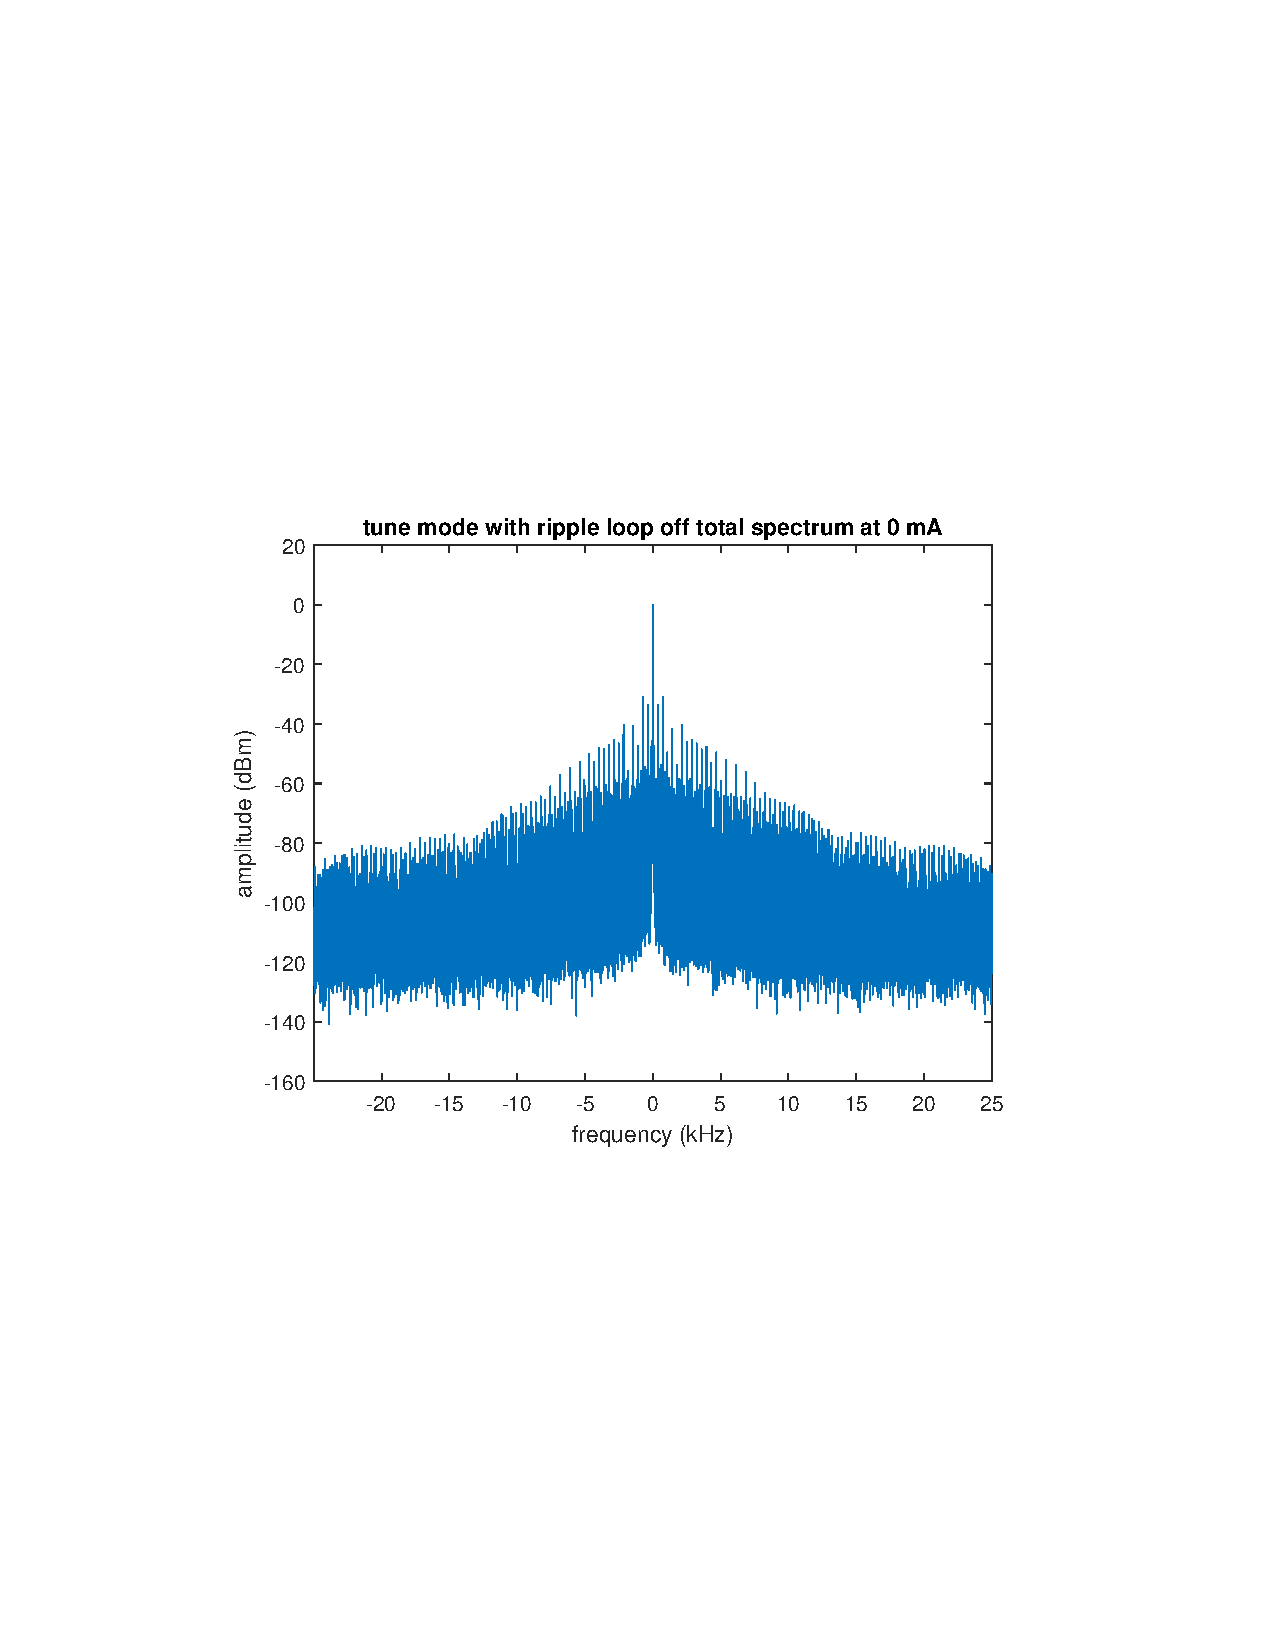
\includegraphics[trim= 3.75cm 8.5cm 3.35cm 8.5cm,clip,width=0.95\linewidth]{graphics/spearCavATuneModeSpectrum.pdf}
		\caption[rawRF]{Spectrum of raw klystron RF output with no feedback provided by the LLRF.}
		\label{fig:rawData}
	\end{figure}
\end{center}

\begin{center}
	\begin{figure}[tbph]
		\centering
		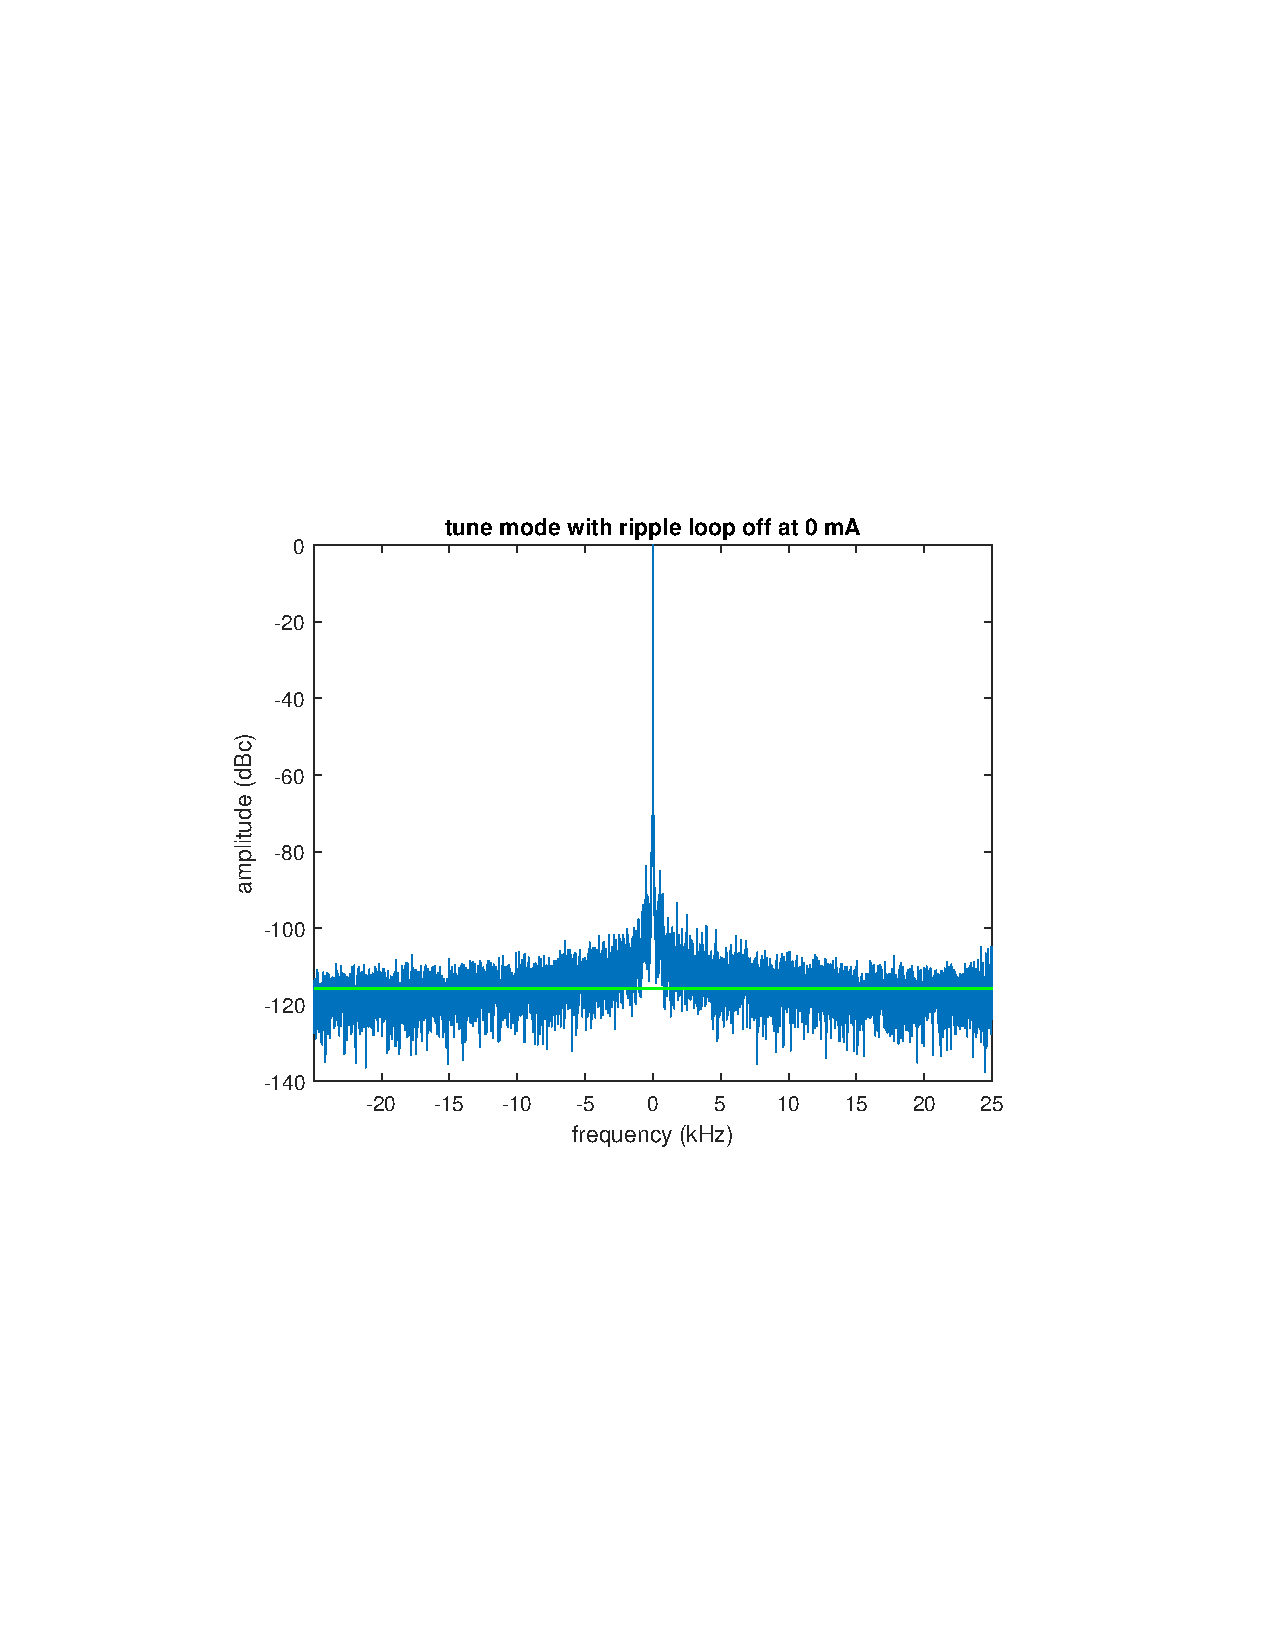
\includegraphics[trim= 3.75cm 8.5cm 3.35cm 8.5cm,clip,width=0.95\linewidth]{graphics/spearCavATuneModeSpectrumFiltered.pdf}
		\caption[rawRF]{Spectrum of raw klystron RF output with no feedback provided by the LLRF, post-processed using our software notch filter.}
		\label{fig:rawDataFiltered}
	\end{figure}
\end{center}

\section{Data Analysis}
\subsection{Methods}
\subsubsection{Power Line Harmonic Suppression}
The measurement of the close-in power line harmonic suppression was straightforward.  We used figure \ref{fig:rawData}, with no current in SPEAR, as the reference for the size of the raw output harmonics and figures \ref{fig:legacyTotal} and \ref{fig:llrf9Total}, with \SI{500}{\mA} in SPEAR, to measure their output when the RF waveform was controlled by the various LLRF systems.  Only the suppression of the dominant \SI{360}{\Hz} and \SI{720}{\Hz} was measured and recorded in Table \ref{tbl:harmonics}.
\begin{table}[hbtp]
	\begin{center}
		\begin{tabular}{|l|r|r|r|r|}
			\hline
			\textbf{Harmonic} & \SI{-720}{\Hz} & \SI{-360}{\Hz} & \SI{360}{\Hz} & \SI{720}{\Hz} \\ \hline
			\textbf{Unfiltered} & \SI{-30.9}{\dBc} & \SI{-33.6}{\dBc} & \SI{-33.6}{\dBc} & \SI{-30.9}{\dBc} \\ \hline
			\textbf{Legacy rejection} & \SI{25.8}{\dB} & \SI{24.9}{\dB} & \SI{27.0}{\dB} & \SI{24.0}{\dB} \\ \hline
			\textbf{LLRF9 rejection} & \SI{16.0}{\dB} & \SI{18.8}{\dB} & \SI{21.3}{\dB} & \SI{20.2}{\dB} \\ \hline
		\end{tabular}
		\caption{Rejection of close-in HVPS generated power line harmonics.}\label{tbl:harmonics}
	\end{center}
\end{table}
\subsubsection{Synchrotron Resonance Properties}
The synchrotron resonance is within the bandwidth of the RF cavities.  Therefore we can measure the parameters of the resonance from the cavity probe signal.  Since this resonance is a damped harmonic oscillator, its response in the frequency domain is that of a Lorentzian.  We fit the center frequencies, strengths, and quality factors of the resonances to the filtered data from the two LLRF systems and present the values in Table \ref{tbl:nus}.
\begin{table}[hbtp]
	\begin{center}
		\begin{tabular}{|l|r|r|r|}
			\hline
			\textbf{Parameter} & \textbf{Frequency} & \textbf{Amplitude} & $ \mathbf{Q} $ \\ \hline
			\textbf{Legacy system} & \SI{8932}{\Hz} & \SI{-92.8}{\dBc} & \ $ 11.1 $ \\ \hline
			\textbf{LLRF9} & \SI{9657}{\Hz} & \SI{-95.9}{\dBc} & \ $ 16.7 $ \\ \hline
		\end{tabular}
		\caption{Lorentzian fit parameters of the $ \nu_{s} $ resonance.}\label{tbl:nus}
	\end{center}
\end{table}
\subsubsection{Noise Floor}
We measured the noise floor in for all systems, raw RF output power and RF output power controlled by both LLRF systems.  In all cases we made these measurements in resonance free areas of the spectra with the power line harmonics removed.  In all cases this measured noise level was about \SI{-112}{\dBm}.

\subsection{Legacy LLRF System}
As stated above, figure \ref{fig:legacyTotal} shows the performance of the legacy system.  One can measure the rejection of the harmonics from the blue trace and measure the rejection of the synchrotron oscillations from the orange trace.  Figure \ref{fig:legacyFiltered} plots only the data after we have passed it through our filter.  The filtered data is also scaled such that the carrier peak is set as the reference and the power amplitude is plotted as decibels below the carrier.

We first see that the legacy LLRF system rejects the \SI{720}{\Hz} by about \SI{25}{\dB} below its level without feedback to a level of about \SI{55}{\dBc}.  However the legacy system appears to introduce a resonance at around \SI{2800}{\Hz}, close to, but not at, the fourth harmonic of \SI{720}{\Hz}.  The width of this peak is significantly broader than the width of a power line harmonic.  These two facts suggest that this peak is an undesired effect of some peaking of the LLRF feedback loop.  There are also lower amplitude distortions that start at about \SI{15}{\kHz}, but these are of lower amplitude and seem to not be part of a resonance.  The beam-induced spectrum in which we are interested, that of \(\nu_{s}\), has an amplitude of about \SI{93}{\dBc} below the carrier.  Its frequency has been lowered from its nominal value and its quality factor is about $ 11 $, so the impedance provided by the legacy LLRF has significant damping effects on the synchrotron resonance.
\begin{center}
	\begin{figure}[tbph]
		\centering
		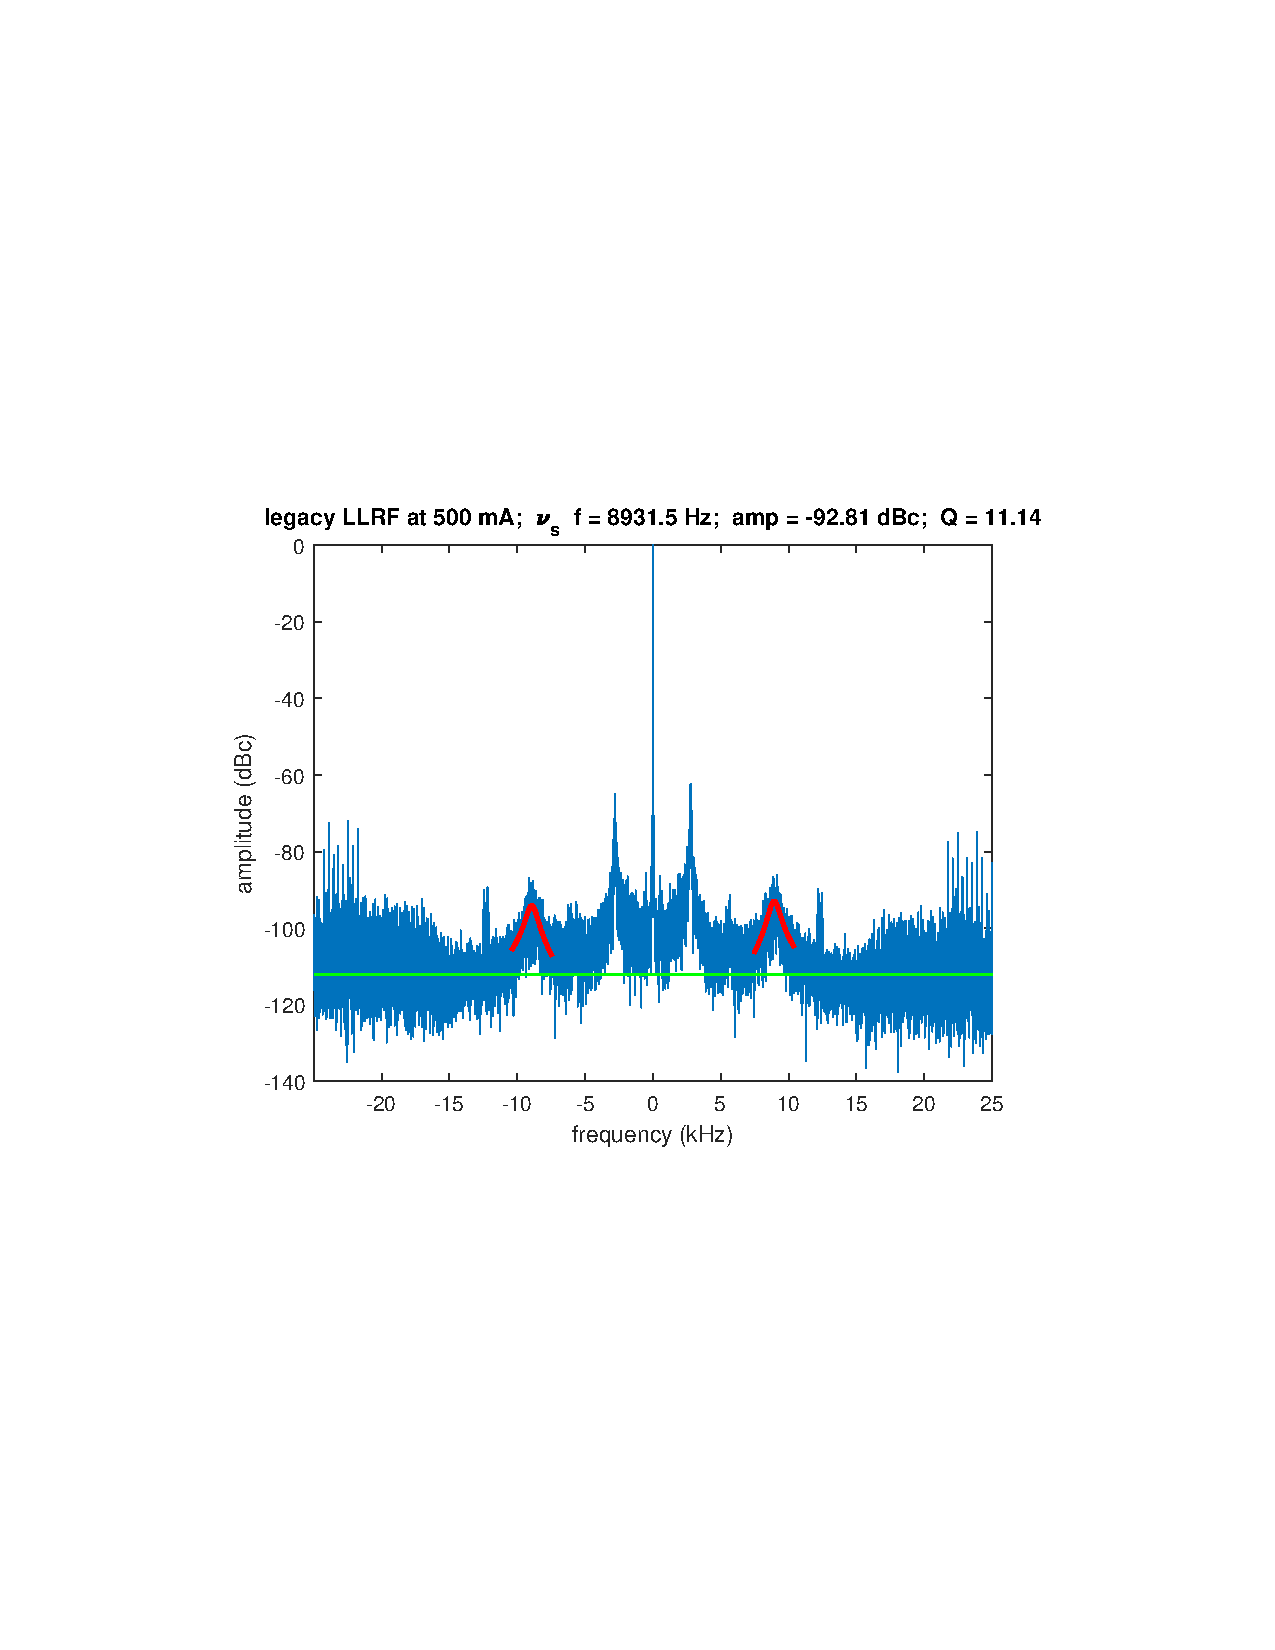
\includegraphics[trim= 3.75cm 8.5cm 3.35cm 8.5cm,clip,width=0.95\linewidth]{graphics/spearCavALegacy500mASpectrumFilteredFit.pdf}
		\caption[legacyFiltered]{Filtered Cavity A spectrum with \SI{500}{\mA} using the legacy LLRF system.}
		\label{fig:legacyFiltered}
	\end{figure}
\end{center}

\subsection{LLRF9 System}
As seen from its spectrum, the LLRF9 outperforms the legacy system in almost every way.  Figure \ref{fig:llrf9Total} combines the raw and filtered data; figure \ref{fig:llrf9Filtered} displays only the filtered data.  The raw data shows that the close-in sidebands generated by the \SI{720}{\Hz} harmonic is about \SI{47}{\dB} below the carrier.  LLRF9 does not do as well as the legacy system in rejecting these close-in harmonics.  This may be due to the special ``ripple loop'' that is part of the legacy LLRF system.

However in all other respects the LLRF9 performance is superior.  The amplitude of the residual synchrotron oscillations is about \SI{96}{\dBc} below the carrier and there is no residual structure generated by the LLRF9.  We note, from both the frequency and quality factor of the synchrotron resonance, that the tuning of the LLRF9 during these experiments did not modify the behavior of the resonance as much as did the legacy LLRF.  The LLRF9 may have the ability to further improve the damping of this resonance.
\begin{center}
	\begin{figure}[tbph]
		\centering
		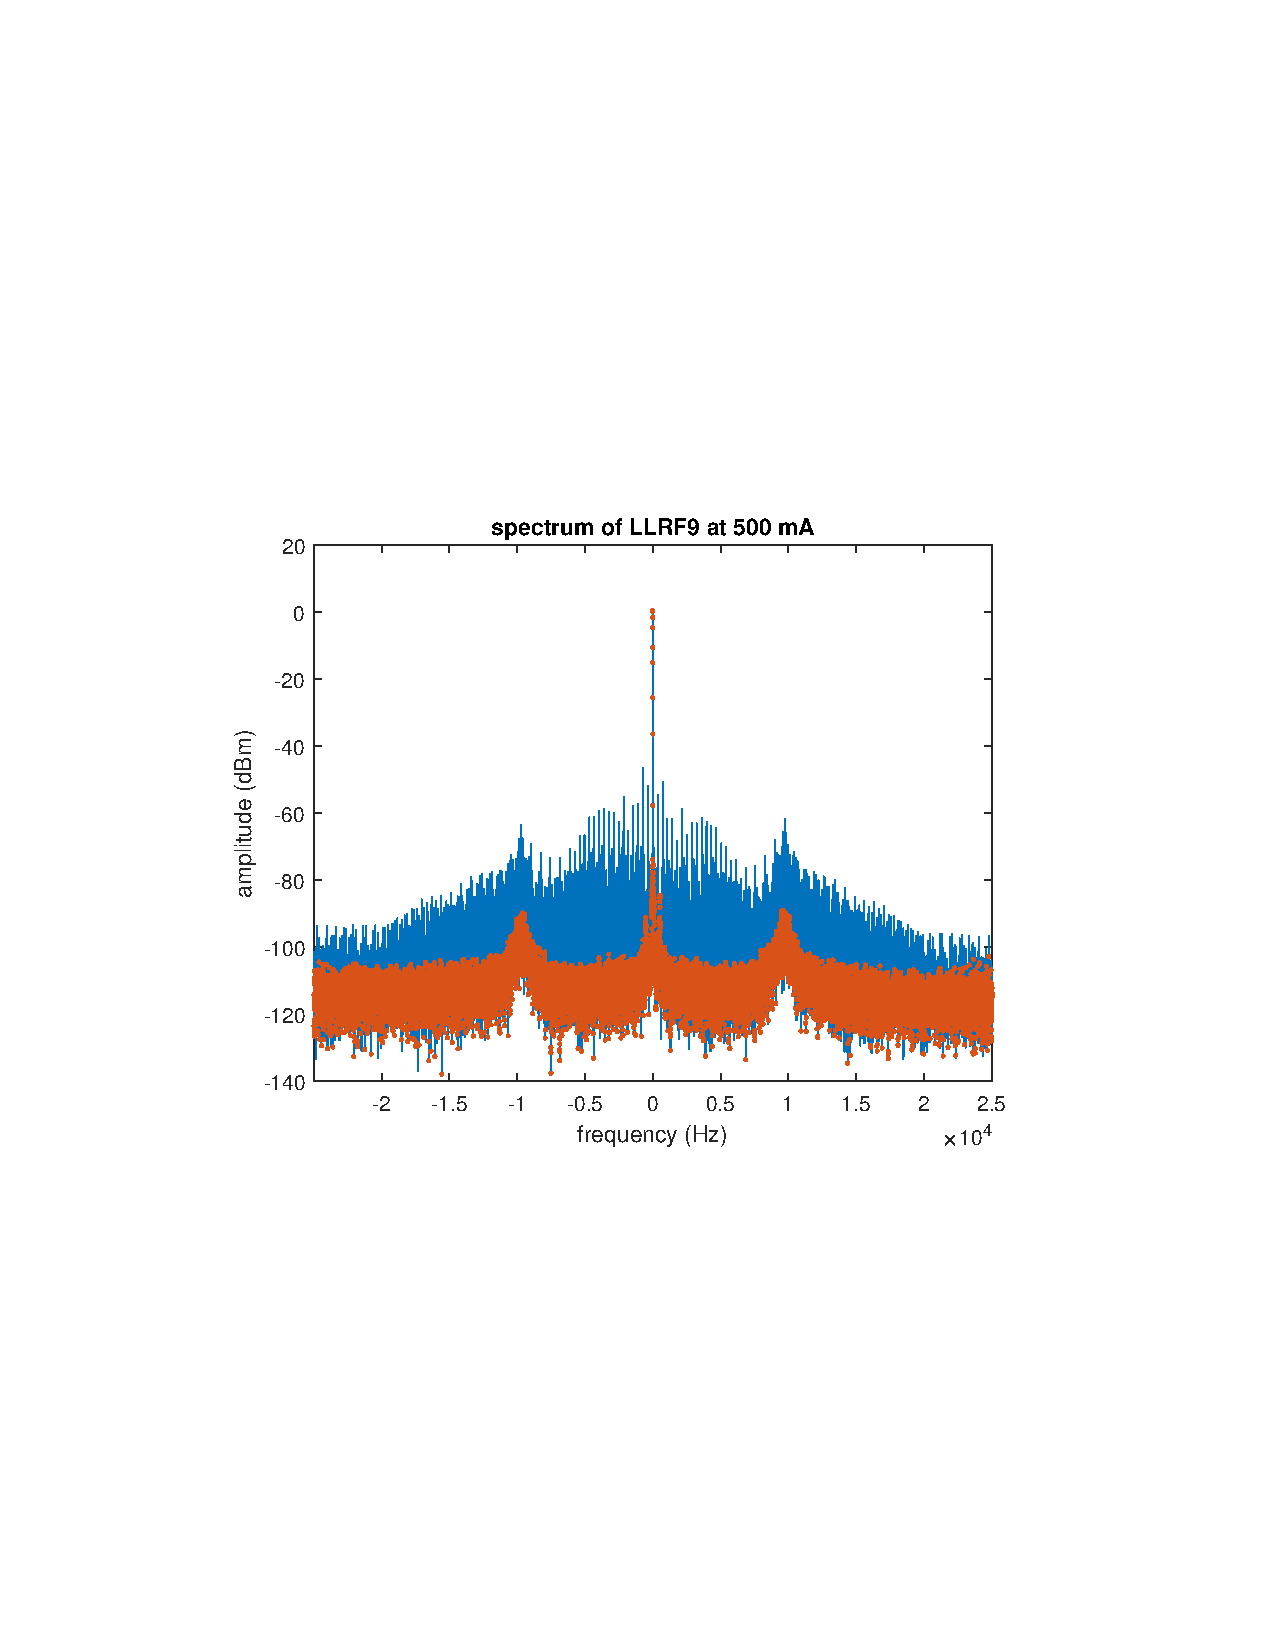
\includegraphics[trim= 3.75cm 8.5cm 3.35cm 8.5cm,clip,width=0.95\linewidth]{graphics/spearLLRF9500Total.pdf}
		\caption[llrf9Total]{Unfiltered and filtered Cavity A spectrum with \SI{500}{\mA} using the LLRF9 system.}
		\label{fig:llrf9Total}
	\end{figure}
\end{center}

\begin{center}
	\begin{figure}[tbph]
		\centering
		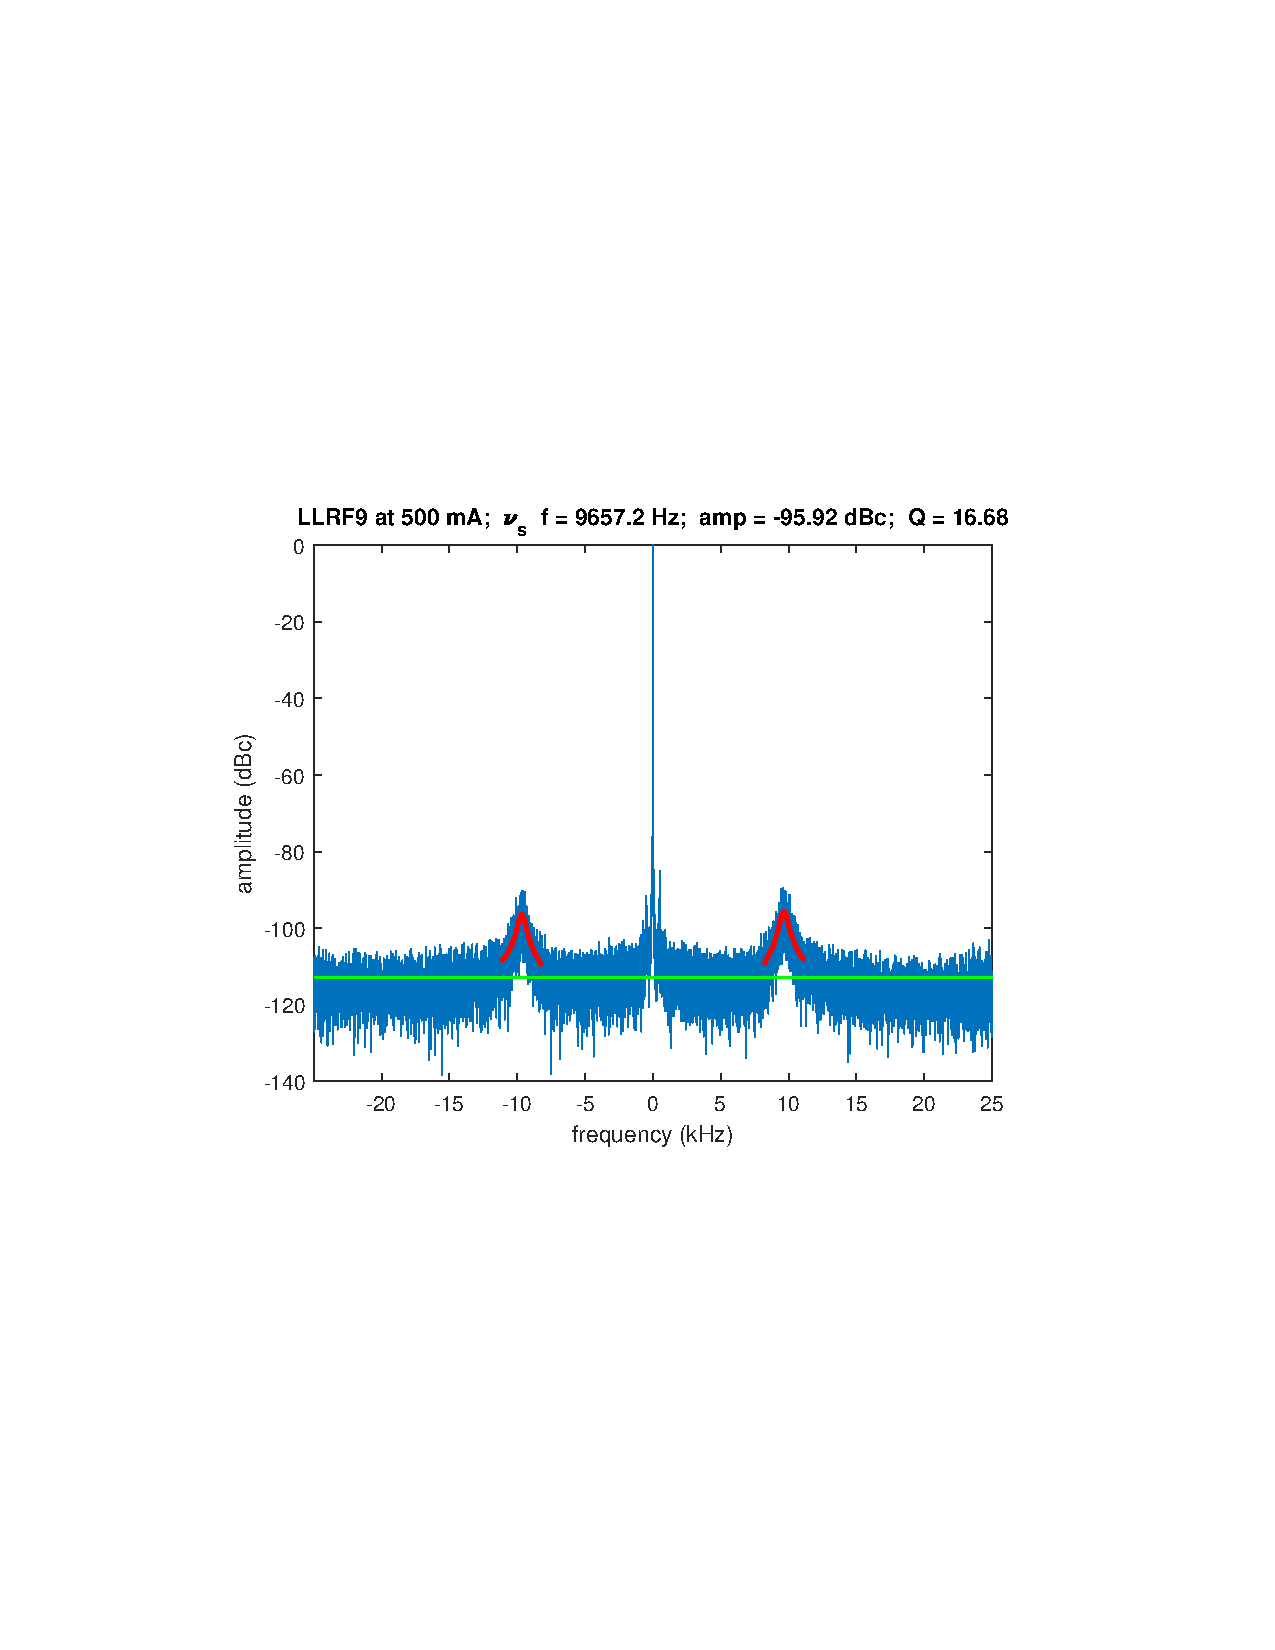
\includegraphics[trim= 3.75cm 8.5cm 3.35cm 8.5cm,clip,width=0.95\linewidth]{graphics/spearCavALlrf9500mASpectrumFilteredFit.pdf}
		\caption[llrf9Filtered]{Filtered Cavity A spectrum with \SI{500}{\mA} using the LLRF9 system.}
		\label{fig:llrf9Filtered}
	\end{figure}
\end{center}


	
% we do not need to insert a \section*{References) line
%\bibliographystyle{IEEEtran}
% need to include full path for .bib file
%\bibliography{/localtexmf/bibtex/bib/sebek}

\end{document}
